\documentclass[a4paper,11pt]{jreport}
\usepackage{masterthesis}
\usepackage[dvipdfmx]{graphicx}
\graphicspath{ {./figure/} }

%次の行を有効にすると、その章だけが読み込まれる
%\includeonly{introduction}

%----------------------------------------------------------------------
% タイトルページ
%----------------------------------------------------------------------
% タイトル 2行にわたる場合は適宜改行をいれること。
\title{拡張現実感を用いた看板画像からの店舗情報アクセス手法に関する研究}

% 提出年月
\date{平成 31 年 2 月}

% 執筆者
\author{北村 茂生}
%----------------------------------------------------------------------


\begin{document}

%タイトルページ
\maketitle

\pagenumbering{roman}
\begin{abstract}

\end{abstract}

%目次
\tableofcontents

%----------------------------------------------------------------------
%本文
%----------------------------------------------------------------------
\newpage
\pagenumbering{arabic}

\chapter{序論}
\label{chapter:introduction}

本章では、本研究の実施に至った背景を説明し、対象とする課題を明確にする。

%------------------------------------------------------------------------
\section{本研究の背景}
\label{section:background}

\chapter{関連研究}
\label{chapter:relatedwork}
本章では,関連研究について述べ,本研究の位置付けを明らかにする.

\section{ARを用いた情報提示に関する研究}
  \subsection{拡張現実感}
    拡張現実感(Augmented Reality; AR)とは,ユーザが見ている現実のシーンに仮想物体を重畳することで,ユーザがいる場所に応じた情報を直感的に提示する技術の総称である\cite{Kambara:2010}.近年,ARを用いたナビゲーションシステムや付加情報提示システムが多数提案されている.ARは主に,Location--based ARとVision--based ARに分類できる\cite{Chatzopoulos:2017}.本研究はVision-based ARを用いる.

  \subsection{ARを用いたナビゲーションに関する研究}
    ARを用いたナビゲーションシステムに関する研究も行われている.
    屋外でのナビゲーションは主にLocation--based ARが用いられており,それに対して屋内でのナビゲーションは主にVision--based ARが用いられている.

    Location--based ARを用いた屋外ナビゲーションシステムの例として,Blippar株式会社\footnote{\url{https://www.blippar.com}(2019/2/5存在確認)}のARCity\footnote{\url{https://itunes.apple.com/us/app/arcity-ar-navigation/id1282527727}\label{footnote:arcity}(2019/2/5存在確認)}が挙げられる.ARCityは,GPSを用いてユーザの絶対位置を特定し,ARKit\footnote{\url{https://developer.apple.com/arkit}(2019/2/5存在確認)}を用いて地形を認識することで,目的地までの道のりを示す矢印をスマートフォンの画面に重畳表示している.
    しかし,このようなLocation--based ARを用いたシステムは,地図上での目的地に到着した後,ユーザが現実世界上で目的地を探す必要がある.
    \begin{figure}[tb]
      \centerline{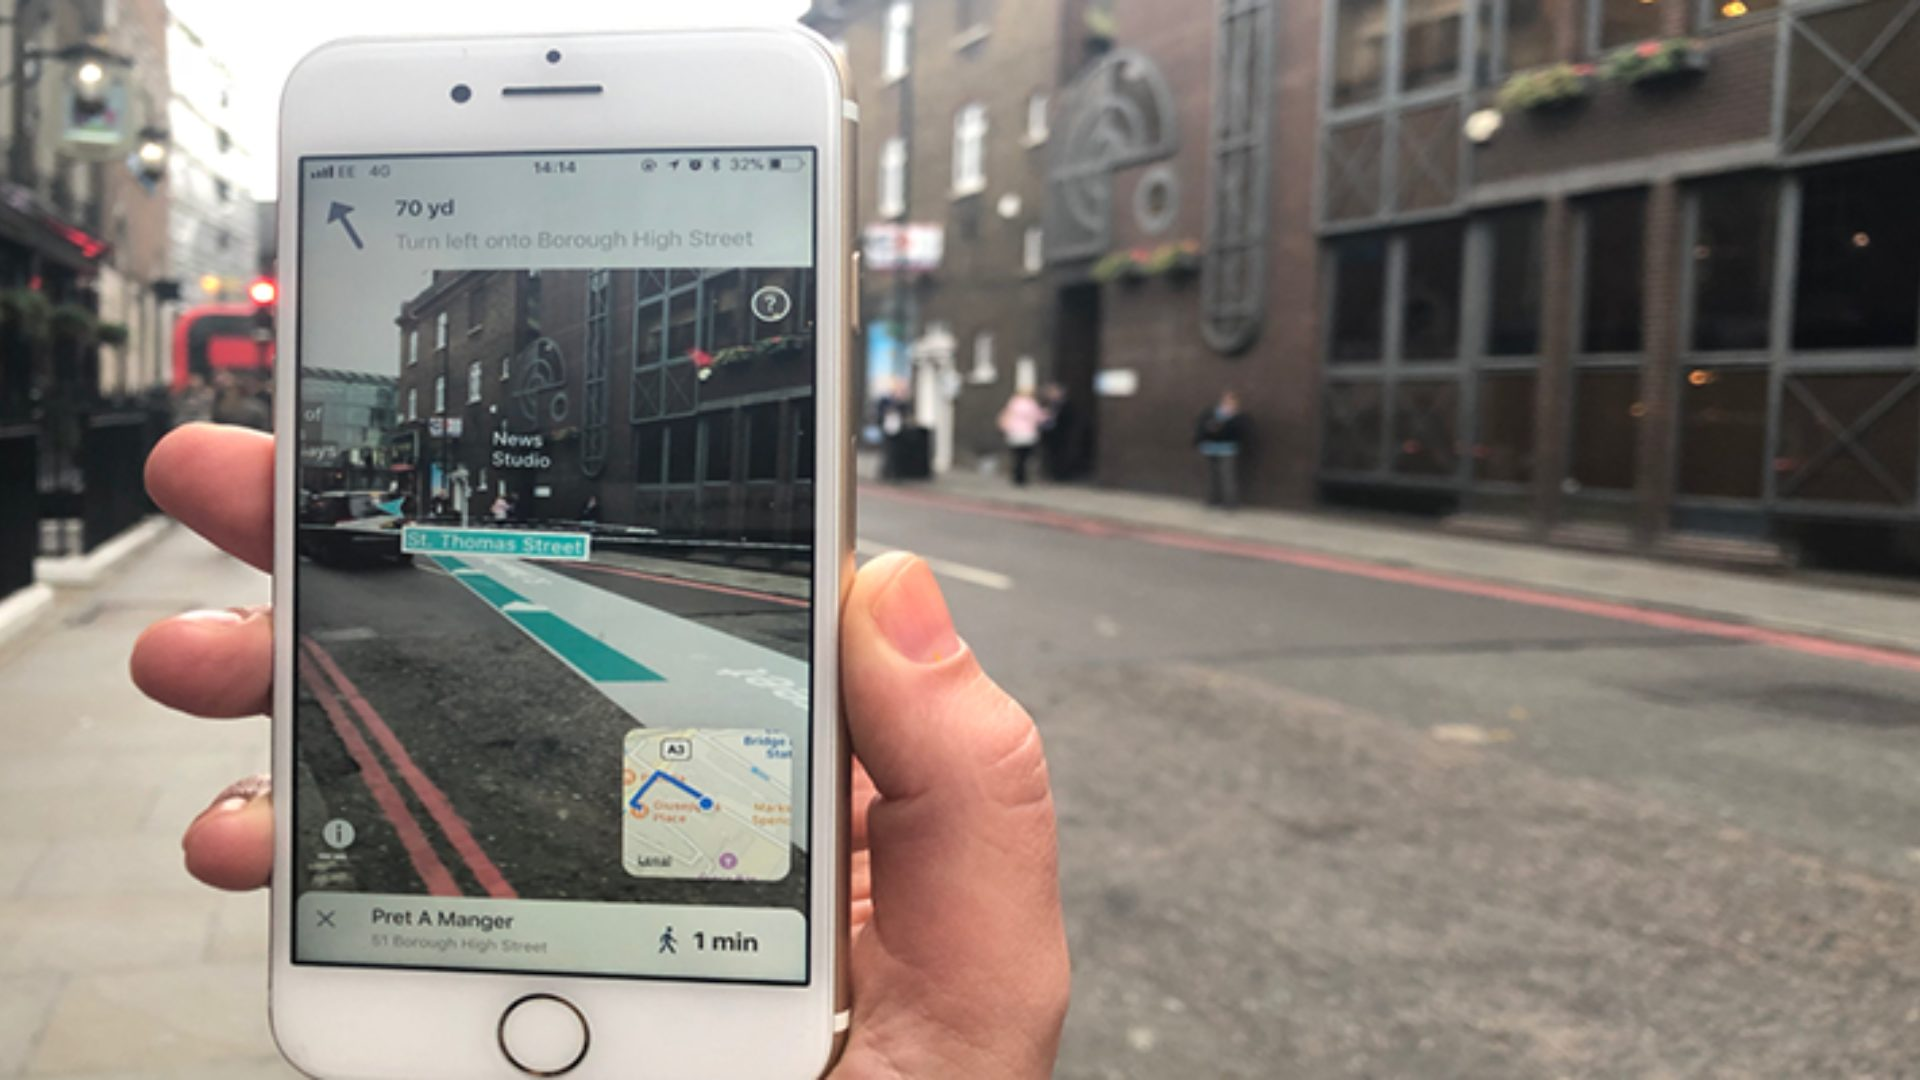
\includegraphics[width=\columnwidth, clip]{arcity.jpg}}
      \caption{(脚注\ref{footnote:arcity}より図引用)}
      \label{figure:koch}
    \end{figure}

    Vision--based ARはさらにマーカ有りとマーカレスに分類できる.
    マーカを用いた屋内ナビゲーションシステムの例として,吉野らは,迷いやすい人の特徴を考慮した上で,QRコードマーカを目印とし,スマートフォン画面上にARで進むべき方向の矢印を表示する屋内ナビゲーションシステム``DoCoKa''を開発している\cite{Yoshino:2013}.
    Kochらは,出口の案内板など自然なオブジェクトをARマーカとしたナビゲーションシステムを開発している\cite{Koch:2014}.これにより,屋内において煙が探知された際に,作動した煙探知機までの経路を提示し,ARを用いて対処方法を提示している.
    \begin{figure}[tb]
      \centerline{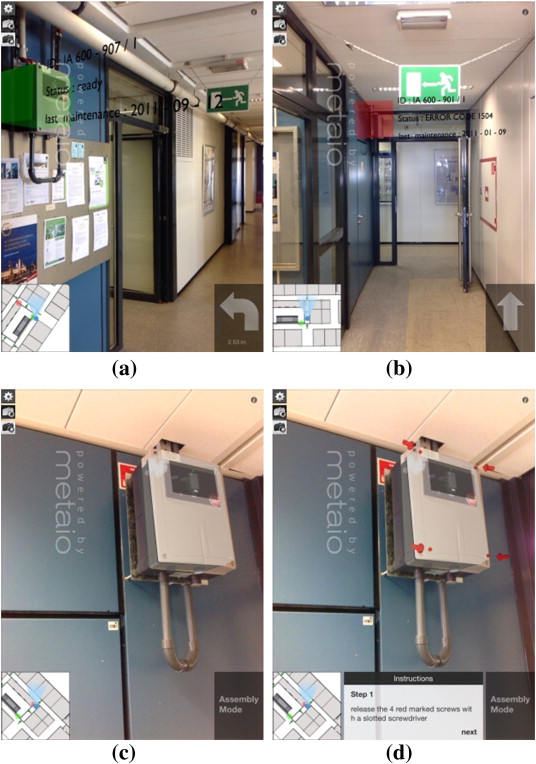
\includegraphics[width=\columnwidth, clip]{koch.png}}
      \caption{(文献\cite{Koch:2014}より図引用)}
      \label{figure:koch}
    \end{figure}

    マーカレスARを用いた屋内ナビゲーションシステムの例として,
    Georgらは,屋内など限定された地域におけるナビゲーションシステムを提案している\cite{Gerstweiler:2018, Iwanaji:2016}.
    しかし,これらのVision--based ARのみを用いたシステムは,屋内など特定の場所でしか利用できない.
    
    このような携帯端末上でのARを用いたナビゲーションは,紙の地図を用いた場合と比較して,より短い時間と少ない操作で目的地まで辿り着けることが明らかとなっている\cite{Rehman:2017, Yoshino:2013}.
    

\section{情報の視認性に関する研究}
  畑らは,画像内に高解像度領域と低解像度領域を作ることによって,ユーザに気づかせることなく視線を特定の領域に誘導させる手法を提案している\cite{Hata:2016}.
  例として,図\ref{figure:hata} --(a)に示す画像をユーザに提示すると,ユーザの視線がどこに集中しているかを示すヒートマップは図\ref{figure:hata} --(b)のようになる.
  \begin{figure}[tb]
    \begin{minipage}{0.49\hsize}
      \begin{center}
        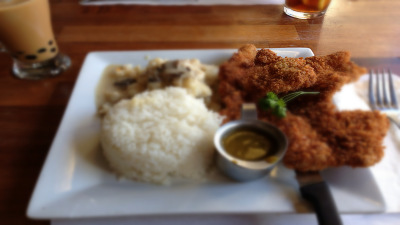
\includegraphics[clip, width=\textwidth]{hata1.png}\\
        \small{(a)提示画像}
      \end{center}
    \end{minipage}
    \begin{minipage}{0.49\hsize}
      \begin{center}
        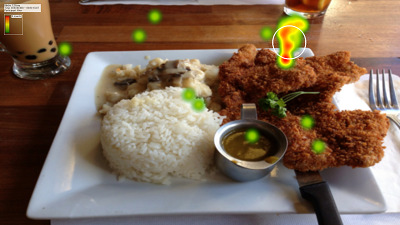
\includegraphics[clip, width=\textwidth]{hata2.png}\\
        \small{(b)ヒートマップ}
      \end{center}
    \end{minipage}
    \vspace{2pt}
    \caption{解像度制御による視線誘導(文献\cite{Hata:2016}より図引用)}
    \label{figure:hata}
  \end{figure}

  拡張現実感とは対称に,隠消現実感(Diminished Reality; DR)の研究が行われている\cite{Mori:2017}.
  DRとは,実世界から図\ref{figure:mori} --(a)のように色情報を取り除いたり,図\ref{figure:mori} --(b)のように物体を透視したり,図\ref{figure:mori} --(c)のように特定の物体を置き換えたり,図\ref{figure:mori} --(d)のように特定の物体を消去したりする技術の総称である.
  \begin{figure}[tb]
    \centerline{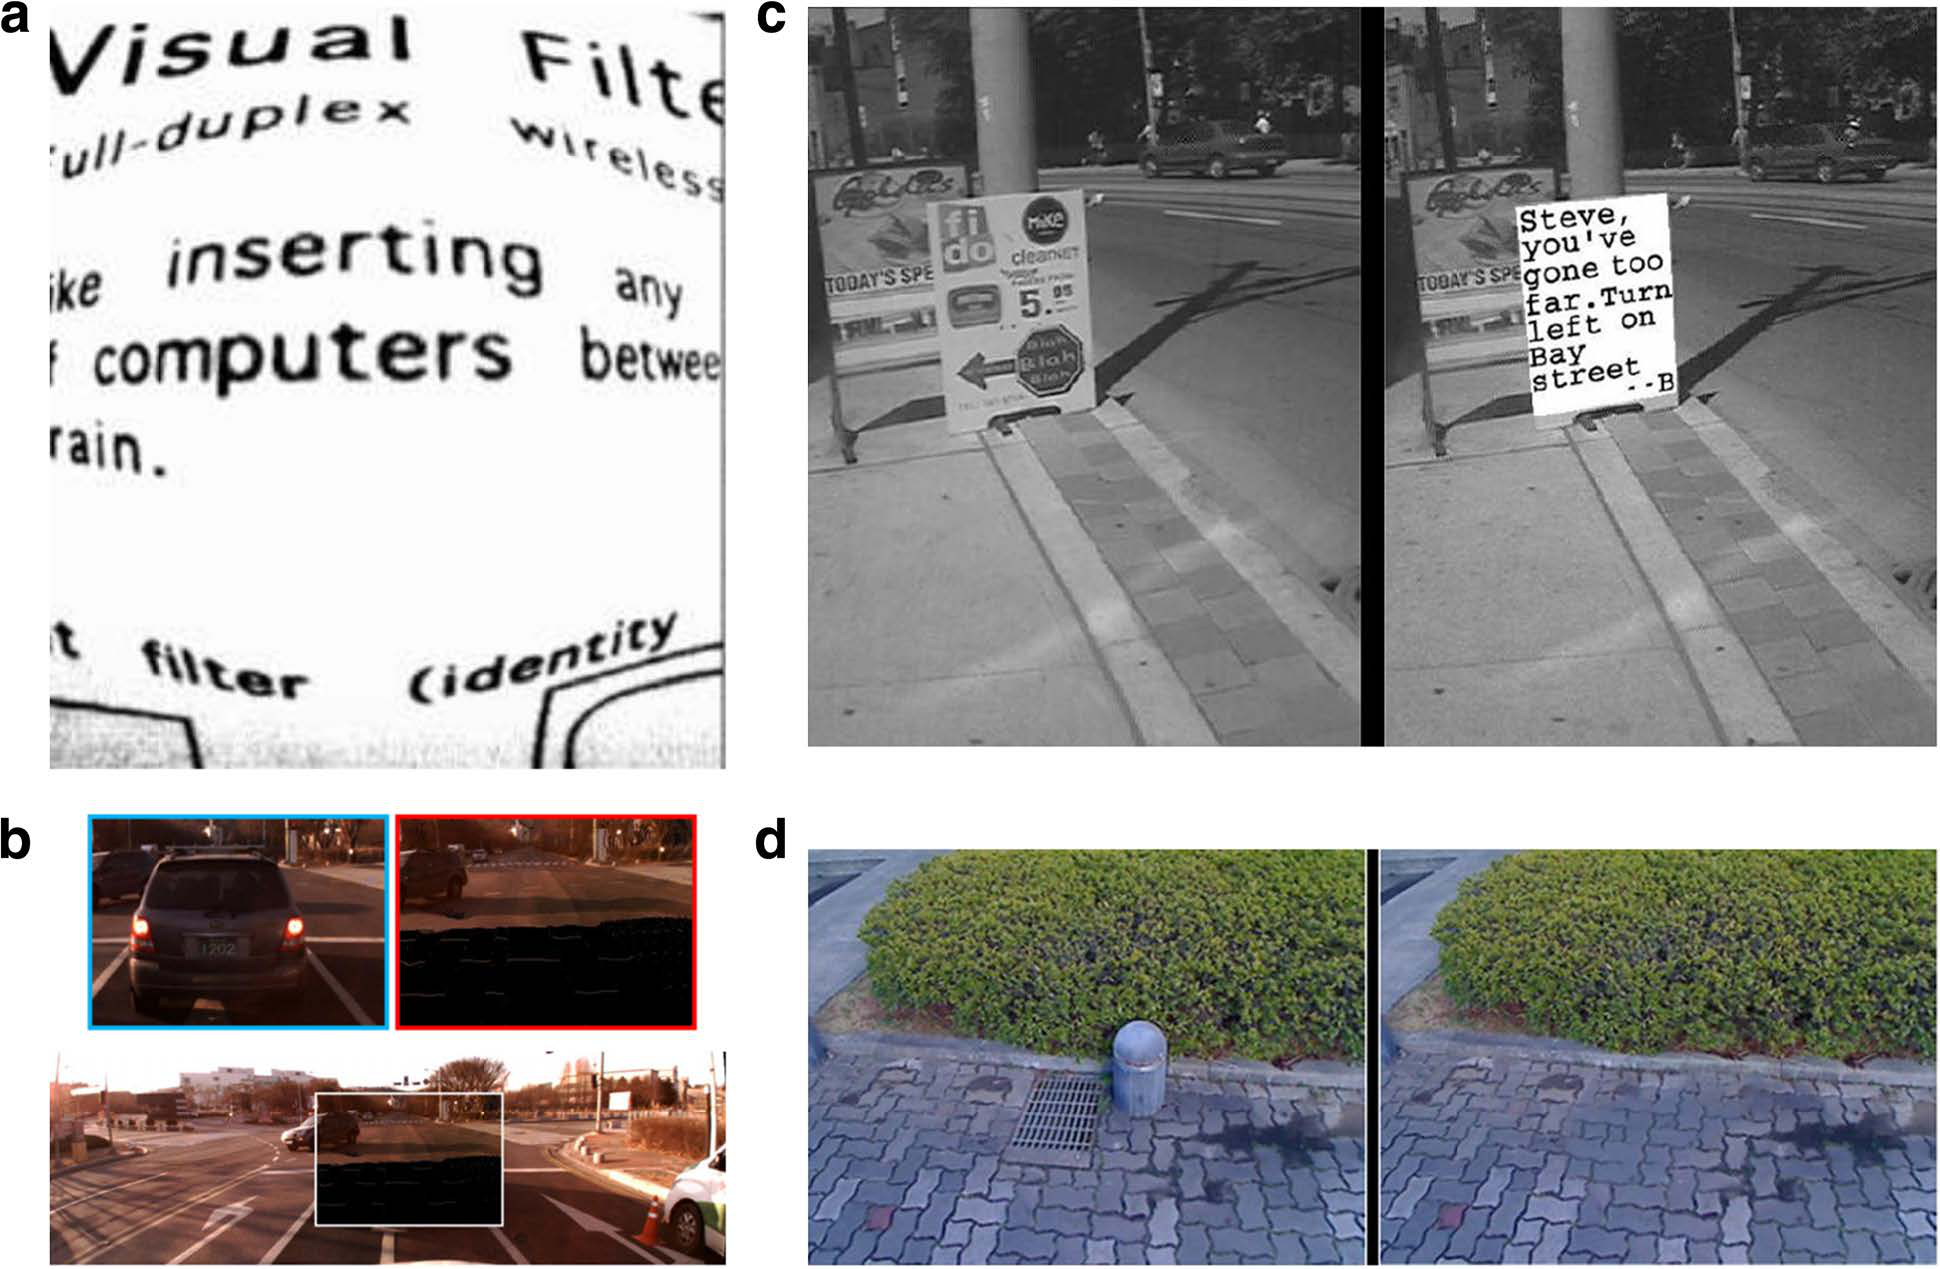
\includegraphics[width=\columnwidth, clip]{mori.png}}
    \caption{隠消現実感(文献\cite{Mori:2017}より図引用)}
    \label{figure:mori}
  \end{figure}

\section{看板認識に関する研究}
  看板に書かれてある文字を認識する研究は多数行われている.
  主な手法としては,ニューラルネットワークを用いて看板に書かれている文字を認識する手法や,Optical Character Recognition(OCR)を用いる手法が挙げられる.
  Heらは,シーケンスラベリング問題として背景から文字を読み取る再帰型ニューラルネットワークを開発している\cite{He:2016}.
  Leeらは,特徴量を用いてストリートビュー画像から文字領域を検出する手法を提案し,OCRソフトウェアが文字認識することを容易にしている\cite{Lee:2016}.
  しかし,看板の中には手書き文字など崩した文字で書かれているものもあり,人間であっても読むことが容易でない場合がある.このような場合は,OCRを用いて文字を認識することは困難である.
  Kavatiらは,図\ref{figure:kavati}のようにスマートフォンで撮影された看板や標識の写真内の文字をOCRによって認識し,英語からテルグ語に翻訳してユーザに提示する旅行者向けのWebアプリケーションを開発している\cite{Kavati:2017}.
  \begin{figure}[tb]
    \begin{minipage}{0.49\hsize}
      \begin{center}
        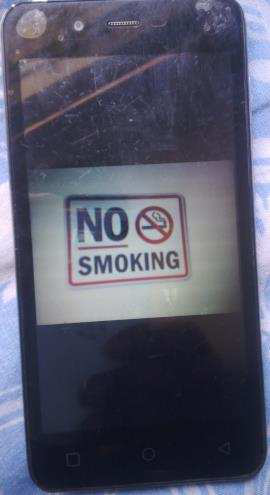
\includegraphics[clip, width=\textwidth]{kavati1.png}\\
        \small{(a)英語}
      \end{center}
    \end{minipage}
    \begin{minipage}{0.49\hsize}
      \begin{center}
        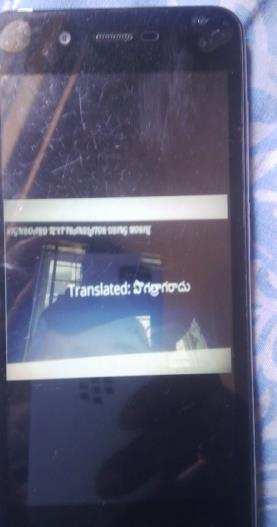
\includegraphics[clip, width=\textwidth]{kavati2.png}\\
        \small{(b)テルグ語}
      \end{center}
    \end{minipage}
    \vspace{2pt}
    \caption{翻訳された看板の文字(文献\cite{Kavati:2017}より図引用)}
    \label{figure:kavati}
  \end{figure}
  
\section{物体認識に関する研究}

\section{本研究の位置付け}

\chapter{提案手法}
\label{chapter:proposal}

\chapter{実験}
\label{chapter:experiment}

\chapter{議論}
\label{chapter:discussion}
本章では,\ref{chapter:experiment_dr}章と\ref{chapter:experiment_sbs}章で述べた実験の結果に基づき,本研究の到達点と改善点,今後の展望について述べる.

\section{得られた知見}
\label{section:obtained_knowledge}
  \ref{chapter:experiment_dr}章で述べた実験では,探索対象が単体であり,時間帯が昼の場合,提案手法であるハイブリッド型情報提示手法は文献\cite{Fujita:2013}で提案された減算型情報提示手法と探索時間に関して有意差は見られなかった.しかし,探索対象が複数の場合及び時間帯が夜で探索対象が単体の場合においては,提案手法は減算型情報提示手法よりも探索時間が有意に短いことが確認された.このことから,背景の彩度が低い場合や複数の看板を探索する場合において,提案手法は有効であると考えられる.また,時間帯が夜で探索対象が複数である場合,加算型情報提示手法と比較して減算型情報提示手法の方が探索時間が長くなる傾向が見られた.これは実験に用いた写真の背景の彩度が低かったこと,新日本新地ビルの看板に白と黒から構成されているものが多く含まれていたことにより,減算の効果が減少したことが原因と考えられる.

  \ref{chapter:experiment_sbs}章で行なった実験の結果から,情報探索時間に関しては,本稿で扱ったいずれの場合においても,提案システムを用いた場合は食べログを用いた場合よりも探索時間が有意に短くなることが明らかとなった.このことから,提案システムを用いることによって,位置情報のみを用いた場合と比較してユーザはより素早く求めている情報を取得することが可能になるといえる.
  情報探索の正確さに関しては,本稿で扱ったいずれの場合においても,提案システムを用いた場合と食べログを用いた場合とでは正解率に有意差は見られなかった.このことから,言語障壁がなければ位置情報のみを用いても正確に情報を探索することが可能であり,提案システムを用いた場合においても正確な情報探索が可能であるといえる.
  さらに,アンケート結果から,提案システムを用いることによって,位置情報のみを用いた場合と比較してより簡単かつ直感的に情報が探索できるようになることが示唆された.

\section{本研究の到達点}
  \ref{chapter:experiment_dr}章で実施した実験では,文献\cite{Fujita:2013}で提案された減算型情報提示手法に文字情報を追加した加算型と減算型のハイブリッド型情報提示手法を提案した.提案手法を用いたシステムのプロトタイプを実装することにより,減算型情報提示手法の問題点であった,不要な情報を減算する際に対象となる看板が白黒であり,かつその周辺の景色の彩度が低い場合に減算の効果が減少するという点が解消されたと考えられる.これにより,彩度が低い環境においても分かりやすい情報提示が可能となった.また,実験結果から看板を探索する際,提案手法を用いることによって探索時間が短くなることが確認された.以上により,\ref{section:purpose}節で述べた看板密集地域における視覚情報の識別性の向上,及び探索時間の短縮が可能になった.

  提案システムを用いることによって,本研究の目的である,ユーザの目の前にある店舗の情報を直感的かつ簡単に取得できることが達成されたと考えられる.
  これにより,?章で述べた,慣れていない地域においても,ユーザが求める条件に合致する店舗を探索できるようになることが示唆された.

\section{改善点}
  \subsection{減算型表示の実環境における実験}
    \ref{chapter:implement_dr}章で実装したシステムは特定の位置で撮影した全天球画像内でのみ店舗の探索が行えるため,\ref{chapter:experiment_dr}章で実施した実験は,人工環境内のみである.そのため,実環境においても本稿で提案した情報提示手法が有用であるかを検証する必要がある.\ref{chapter:implement_recog}章で実装したリアルタイム看板認識APIを用いることにより,実環境での実験が可能になるため,看板が密集している地域においてOSMのデータベースと看板データベースを構築し,実環境において提案手法の優位性を検討する.

  \subsection{看板認識手法}
    \ref{chapter:implement_recog}章で実装したシステムの改善点として,(1)OSMのノードと看板画像を手作業で関連付けなければならない点,(2)インターネット上の情報から多種多様な店舗の看板画像を大量に集めることは困難であるため,手作業で看板画像を1店舗につき100枚程度集めなければならない点,が挙げられる.
    (1)に対しては,看板画像を提示してユーザに店舗名を回答するシステムを実装することで解決でき,(2)に対してはユーザに店舗の看板画像を提示し,それと同じ写真を撮影して投稿するシステムを実装することで解決できると考えられる.
    これらのシステムにゲーミフィケーションを利用し,ユーザの行動に対して報酬を与えることによって,多数のデータを効率よく収集できると考えられる.
    
    今後の展望として,看板認識をサーバ上で行うのではなく,Tiny--YOLO等を用いて携帯端末上で行うことを検討する.これにより,サーバへ画像を送信する必要がなくなるため,通信量の大幅な軽減が期待される.

  \subsection{対象地域の拡張}
    \ref{chapter:experiment_sbs}章で
    OSMのデータは誰もが編集可能であるため,その地域に慣れている地元のユーザが自身でデータを収集し,OSMを通して活用できるようになる枠組みの構築を目指す.
    OSMのノードには``cuisine''タグが存在し,``burger'',``noodle'',``japanese'',``chinese''など,飲食店で提供される食品の種類を表す値を追加できる.他にもベジタリアン向けのメニューが提供されていることを表す``diet:vegetarian''や,イスラム教の戒律で許されている食品のみを使用したメニューが提供されていることを表す``diet:halal''などのタグも存在する.
    さらに,店舗名の英語またはローマ字表記を表す``name:en''タグや中国語表記の``name:zh''タグ,韓国語表記の``name:ko''タグなどを充実させることによって,ユーザインタフェースを多言語に対応させることが可能となる.
    これらのデータを活用することにより,その地域に慣れていない人や,地元の文字が読めない外国人観光客に対して,求めている情報を容易に取得でき,アレルギーや宗教的制約などの理由による食事制限にも対応可能なナビゲーションを実現できる.
    
    本稿における実験参加者は地元の大学生であるため,地域に慣れていないユーザや非漢字圏など地元の文字が読めないユーザを対象としたユーザ実験を実施する.
\chapter{結論}
\label{chapter:conclusion}
  本研究の目的は,ユーザが慣れていない地域や周囲の文字が読めない状況であっても,目の前にある店舗の情報を直感的かつ簡便に取得できるシステムの実現である.
  本稿では「周囲に看板が多数存在する状況」と「周囲の文字が読めない状況」を対象としたプロトタイプを実装し,ユーザ実験を行うことで,既存のシステムとの差異を明らかにした.
  以下の本稿の内容を纏める.

  \ref{chapter:introduction}章では,本研究に至った背景と問題点を述べ,解決すべき課題を明らかにした.
  街中における店舗の看板は,人々が求める条件に合致した店舗を探す際に重要な役割を果たしている.
  しかし,街中における情報探索の問題点として(1)繁華街など看板が密集している地域においては,大量に存在する他の視覚情報に紛れて目的の看板を見つけることが出来ない可能性があること,(2)外国人観光客の場合,言語障壁により目の前にある店舗が自身の求める条件に合致するか検索することが困難である点,の2点を挙げた.
  (1)に対しては,ユーザにとって不要な情報を目立たなくさせ,必要な情報には追加情報を重畳表示すること,(2)に対しては,スマートフォンのカメラを通して店舗の看板を見るとカメラ映像上に店舗の詳細情報が得られるシステムを実装することにより,これらの問題を解決すると述べた.
  これらの提案手法の優位性を検証するために,従来手法と比較したユーザ実験を行うことを述べた.

  \ref{chapter:relatedwork}章では,本研究で提案するシステムの実現に関連する研究を述べ,本研究の位置付けを明らかにした.
  まず,ARを用いたナビゲーションシステムについて説明し,ARを用いることで紙の地図を用いる場合と比較してより少ない時間で目的地まで辿り着けることについて述べた.
  次に,情報の視認性に関する研究として,解像度制御による視線誘導と,隠消現実感について述べた.
  続いて,看板認識に関する研究として,OCRを用いて看板に描かれている文字を認識する研究や,物体検出に関する研究として,CNNを用いて画像の中から物体領域を検出する研究について述べた.
  最後に,本研究の位置付けとして,Vision-based ARを用いることと,CNNを用いて看板を認識することを述べた.

  \ref{chapter:design_guidline}章では,これまでの取り組みとして,減算型表示について説明し,本研究で対象とする状況及び提案システムの要件について述べた.
  加えて,提案システムの要件を満たすための前提条件と,本稿の提案手法であるSearch by Snapについて説明し,そのインタフェースのデザインについて述べた.

  \ref{chapter:implement_dr}章では,減算型表示を用いたプロトタイプの実装について述べた.
  プロトタイプでは,ユーザはモバイルデバイスを全天球画像内で全方向に向けることができ,選択されていない種類の店舗の視覚情報を減算すると述べた.

  \ref{chapter:implement_recog}章では,リアルタイムで看板認識を行うために実装したAPIについて述べた.
  (1)YOLOv2を用いて看板領域を検出し,(2)VGG16を用いて看板を分類することにより,画像内の看板を認識することを述べた.
  リアルタイムで看板認識を行うために,GPUを搭載したマシン上にWeb APIサーバを構築し,モバイルデバイスからAPIを呼び出すことでリアルタイム認識を実現した.

  \ref{chapter:implement_sbs}章では,\ref{chapter:design_guidline}章で述べたデザイン指針に基づき,Search by Snapを用いて実装したプロトタイプについて述べた.
  \ref{chapter:implement_recog}章で実装したAPIと,OpenStreetMapのデータベースに格納されている店舗情報を用いることによって,ユーザがモバイルデバイスのカメラを通して店舗の看板を見ると,その店舗の情報が得られるシステムを実装した.

  \ref{chapter:experiment_dr}章では,\ref{chapter:implement_dr}章で実装したプロトタイプを用いて実施した評価実験について述べた.
  実験参加者には,全天球画像内で指示された看板を探索するタスクを課した.
  実験の結果,ユーザにとって不要な視覚情報を減算し,必要な情報には付加情報を重畳表示することによって,探索時間が有意に短くなることを示した.

  \ref{chapter:experiment_sbs}章では,\ref{chapter:implement_sbs}章で実装したプロトタイプを用いて実施したユーザ実験について述べた.
  実験参加者には,実際の商店街において,ユーザが条件に合う店舗を探している状況を想定し,使えるクレジットカードの種類と月曜日の営業開始時刻を調べるタスクを課した.
  提案システムと位置情報を用いた検索サービスとを比較した結果,探索時間に関しては提案システムを用いることで有意に短くなることを示し,正解率に関しては有意差がなく,どちらも正確に探索ができることを示した.

  \ref{chapter:discussion}章では,\ref{chapter:experiment_dr}章及び\ref{chapter:experiment_sbs}章で実施した実験から得られた知見と本研究の到達点,提案システムの改善点を述べた.
  本稿で提案した2つのシステムを用いることによって,ユーザが慣れていない地域においても,ユーザが求める条件に合致する店舗を探索できるようになることが示唆された.
  改善点としては,(1)\ref{chapter:implement_dr}で実装したプロトタイプを実環境でも利用できるよう新たに実装を行う点,(2)看板認識に必要なデータセットを効率よく収集する手法を確立する点,(3)OSMのデータベースの充実やインタフェースを多言語化する点,の3点が挙げられる.

  \ref{chapter:conclusion}章では,本稿の要点をまとめ結論づけた.
\chapter*{謝辞}
全ての人と馬に感謝いたします.

\bibliographystyle{ipsjsort}
\bibliography{bibsample}


\end{document}